\subsection{Etherless-smart}
\subsubsection{Struttura}
  Il compito del modulo etherless-smart é di:
  \begin{itemize}
    \item gestire la comunicazione tra gli altri due moduli che compongono il prodotto\ped{\textit{G}};
    \item gestire il pagamento per le operazioni eseguite dagli utenti sulla piattaforma \textit{Etherless}.
  \end{itemize}
  Per implementare queste funzionalitá abbiamo sviluppato i seguenti smart contract:
  \begin{itemize}
    \item \textbf{EtherlessSmart:} gestisce la comunicazione con con gli altri due moduli rendendo pubblici alcuni metodi e attraverso l'emissione di eventi sulla rete; comunica anche con gli altri due contratti sotto descritti come supporto alle operazioni di pagamento e di lettura e scrittura dei dati relativi alle funzioni;
    \item \textbf{EtherlessStorage:} gestisce la memorizzazione e la lettura dei dati delle funzioni sulla rete Ethereum;
    \item \textbf{EtherlessEscrow:} contratto di supporto per permettere la gestione dei pagamenti in modalitá escrow con l'eventuale restituzione dei fondi all'utente.
  \end{itemize}
\subsubsection{Design}
  Il modulo etherless-smart é stato progettato con lo scopo di ridurre per quanto possibile il costo delle transazioni, eliminandolo dove possibile per le operazioni che richiedono la sola lettura dei dati dal contratto. A questo scopo tutte le funzioni che non modificano la memoria interna del contratto sono contrassegnate con il modificatore \texttt{view}, indicando al compilatore che il metodo non modifica lo stato del contratto.
  Durante la progettazione abbiamo fatto riferimento ai seguenti design pattern per il linguaggio Solidity:
  \begin{itemize}
    %%\item \textbf{Memory Array Building:} per mantenere e scorrere i dati relativi alle funzioni memorizzati in EtherlessStorage nel modo piú efficiente possibile abbiamo implementato un mapping \texttt{availableFunctions}, che mette in relazione i nomi della funzione alla struct \texttt{jsFunction}, permettendo un accesso diretto alle informazioni di una funzione conoscendone il nome; inoltre abbiamo utilizzato un array \texttt{functionNames} che permette un'iterazione semplice sulla "lista" di funzioni memorizzate.
    \item \textbf{Access Restriction:} alcune funzioni messe a disposizione nel modulo etherless-smart in diversi contratti devono essere pubbliche, perché devono essere chiamate dall'esterno del contratto stesso (da un altro contratto o dal modulo etherless-server), tuttavia questo implica che possono essere chiamate da chiunque interagisca con la rete Ethereum. Quindi per motivi di sicurezza l'accesso a queste funzioni deve essere limitato ad indirizzi specifici:
      \begin{itemize}
        \item le funzioni di pagamento del contratto EtherlessEscrow devono essere disponibili solo per il contratto EtherlessSmart; questa funzionalitá é ottenuta attraverso una derivazione dal contratto \texttt{Ownable} offerto da OpenZeppelin;
        \item le funzioni di risposta (come \texttt{runResult}, \texttt{deployResult}, etc.) devono essere chiamate solo da etherless-server; questa funzionalitá é ottenuta implementando un modificatore apposito \texttt{onlyServer}.
      \end{itemize}
    \item \textbf{Secure Ether Transfer:} il trasferimento di ether da un indirizzo ad un'altro é gestito in modo sicuro dal contratto EtherlessEscrow, che nelle funzioni di trasferimento dei fondi utilizza il metodo \texttt{sendValue}, fornito dal contratto \texttt{Address} offerto da OpenZeppelin;

    \item \textbf{String Equality Comparison:} Solidity non offre funzionalitá di comparazione tra stringhe, quindi abbiamo costruito un metodo apposito \texttt{compareString} che si occupa di verificare l'uguaglianza tra due stringhe. Per rendere questa operazione meno costosa in termini di gas, abbiamo seguito il pattern String Equality Comparison, che comporta, oltre al confronto per carattere, un previo confronto tra la lunghezza delle stringhe evitando controlli inutili e dispendiosi;
  \end{itemize}

  \paragraph{Proxy e contratti upgradable}
    Generalmente i contratti caricati su rete Ethereum sono immutabili, ovvero il loro codice implementato non puó variare. OpenZeppelin fornisce una funzionalitá di "upgrade" per gli smart contract che funziona attraverso un meccanismo di proxy giá incluso nello strumento, semplificando la gestione dell'aggiornamento del codice dei contratti.
    I contratti EtherlessSmart e EtherlessStorage sono stati implementati in modo da poter sfruttare questo meccanismo, il quale ad una richiesta di upgrade di un contratto caricato sulla rete ad un certo indirizzo, si occupa di "reindirizzarlo" in modo da mantere lo stesso indirizzo sulla rete Ethereum ma non riferendosi piú alla implementazione originale del contratto, bensí a quella aggiornata.

\newgeometry{a4paper,left=1in,right=1in,top=1in,bottom=1in,nohead}
\begin{landscape}
\subsubsection{Diagramma delle classi}
  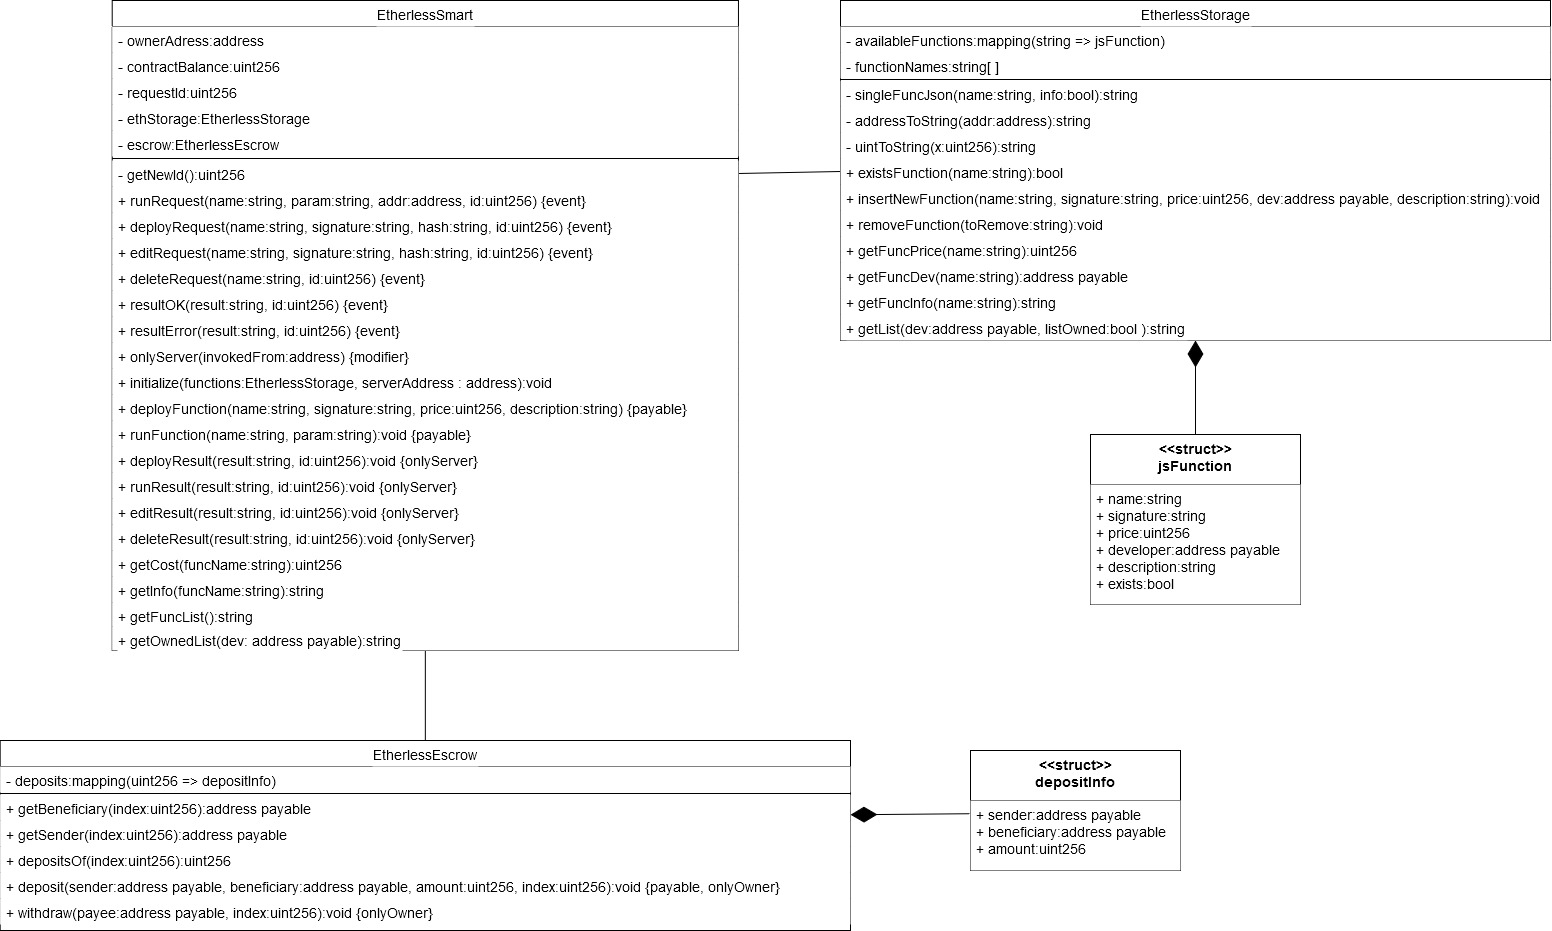
\includegraphics[width=21.5cm, height=14cm]{././diagrammi/etherless-smart/classi/Etherless-smart.jpg}
\end{landscape}
\subsubsection{Diagramma di sequenza}
\subsubsection{Diagramma di attività}
